\section{Durchführung}
    \label{sec:Durchführung}
    Die Wärmepumpe wird wie in Abbildung \ref {fig:aufbau} zu sehen aufgebaut. 
    Zuerst werden die beiden Reservoire mit jeweils circa 3 Liter Wasser befüllt.
    Daraufhin werden die Rührmotoren eingeschaltet, welche dafür sorgen,
    dass die Temperatur in beiden Reservoiren möglichst homogen über das gesamte Volumen im jeweiligen Reservoir verteilt ist.
    Nach der Aktivierung des Kompressors gilt es im 1-Minutentakt die aufgenomme Leistung vom Kompressor P, abzulesen am Wattmeter,
    sowie den Druck $p_\text{1,2}$ und die Temperatur $T_\text{1,2}$ des zugehörigen Reservoirs (vgl. Abbildung \ref {fig:aufbau})
    vom Mano- bzw. Thermometer abzulesen und zu notieren. Die Messreihe wurde beendet nachdem die Temperatur des zu heizenden Reservoirs 50°C übersteigt.
    \begin{figure}
        \centering
        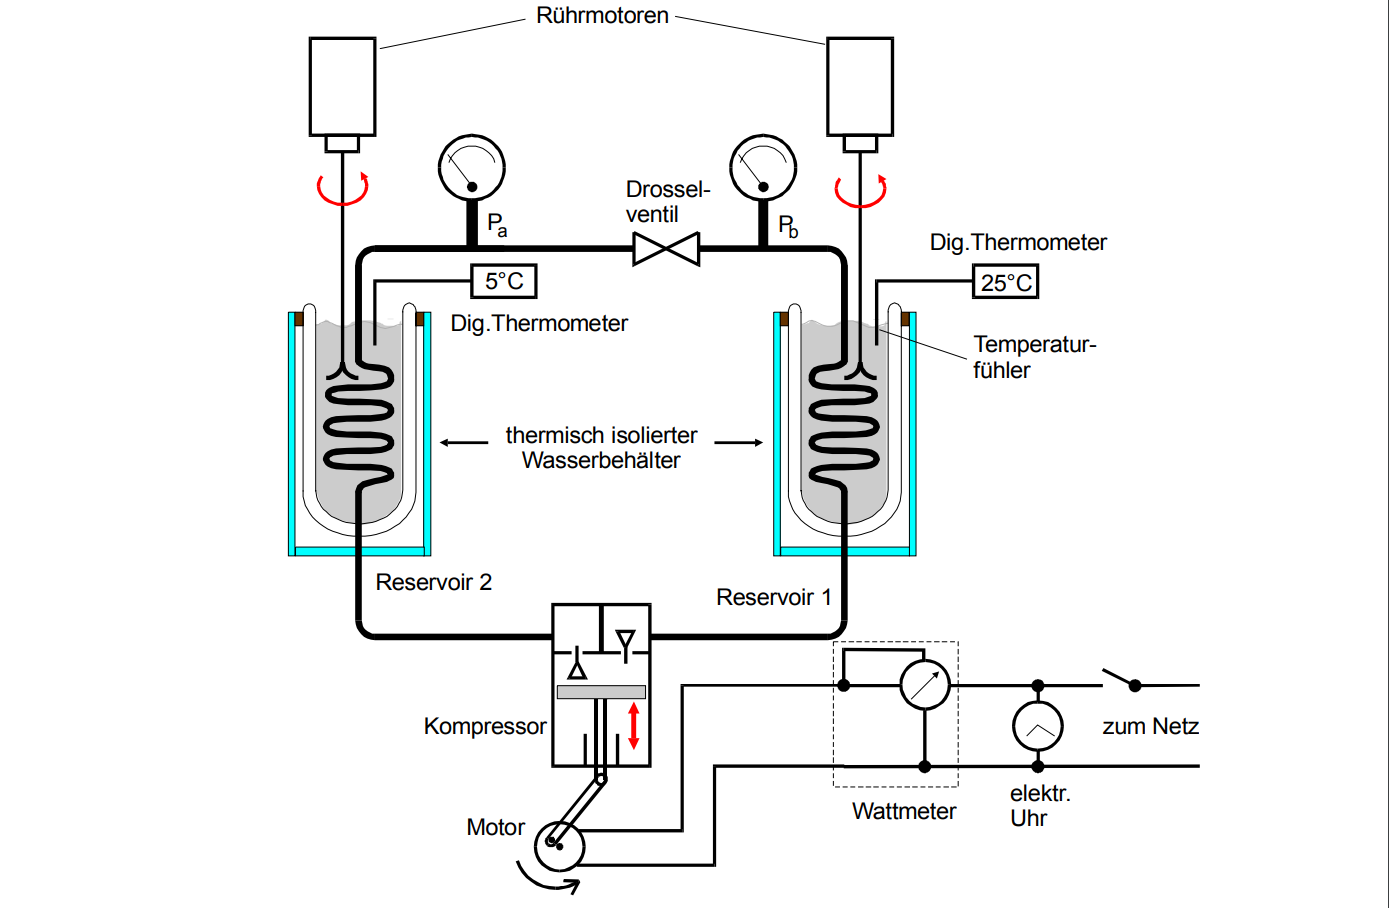
\includegraphics[width=\textwidth]{content/aufbau.png}
        \caption{Aufbau der Messaparatur \cite[197]{206}}
        \label{fig:aufbau}
    \end{figure}